\documentclass[useAMS,usenatbib]{mn2e}

\usepackage{amsmath,amssymb}
\usepackage{graphicx}
\usepackage{epstopdf}
\usepackage{color}
\usepackage[normalem]{ulem}
\usepackage[usenames,dvipsnames]{xcolor}
\usepackage{aas_macros}
\usepackage{url}

\newcommand{\lal}{Lyman-$\alpha$ }
\newcommand{\lab}{Lyman-$\beta$ }
\newcommand{\siiv}{Si~{\small IV} }
\newcommand{\oone}{O~{\small I} }
\newcommand{\cfour}{C~{\small IV} }
\newcommand{\ctwo}{C~{\small II} }
\newcommand{\sfour}{Si~{\small IV} }
\newcommand{\nfive}{N~{\small V} }
\newcommand{\magtwo}{Mg~{\small II} }

%\author[Bosman \& Codoreanu]
%  {Sarah E. I. Bosman$^{1}$, Alex Codoreanu$^{2}$
%\\
%% List of institutions
%$^{1}$ Department of Physics and Astronomy, University College London, Gower Street, London WC1E 6BT, UK \\
%$^{2}$ Centre for Astrophysics and Supercomputing, Swinburne University of Technology, Hawthorn, Victoria 3122, Australia \\
%$^{3}$ ARC Centre of Excellence for All-sky Astrophysics (CAASTRO)
%}


\title{Physical sizes of Mg~II haloes beyond $z=5$: a statistical study}

\date{}
\begin{document}
\maketitle

\begin{abstract}
We present a simple analytical model for constraining the sizes of \magtwo regions around young galaxies at $5<z<7$. Using a compilation of recent high-redshift measurements, we find that enriched regions around bright ($M_\text{AB} = -18$) galaxies must have sizes $R<200 cMpc$ to remain consistent with both the luminosity function of galaxies and occurrence rates of intervening absorbers towards background quasars. At the same time, we find that the lack of confirmed galaxy-absorber pairs in the fields around background quasars strongly implies a limiting magnitude of enrichment $M_\text{min}>-19$. This result might help guide observational attempts to find such galaxy-absorber pairs. Finally, we produce a chart of smallest enriched region size versus choice of limiting magnitude for enrichment, which might be of use for numerical models of metal enrichment as a guide for required resolution.
\end{abstract}

\section{Introduction}

%Using an analytical model and a compilation of recent high-redshift measurements, it is now possible to put surprisingly tight constraints on the extents of Mg II regions around young galaxies. These constraints might help guide simulations, which struggle to reproduce the observed occurrence rates of Mg II. They also have (slightly saddening) implications for observations which are attempting to find galaxy-absorber pairs towards high-redshift quasars.

Metal enrichment in the circum- and meta-galactic medium is a leading probe of galaxy evolution.
At low and intermediate redshifts, the composition of metal-enriched gas studied in the emission and absorption has yielded unique insight into the nature of galactic inflows and outflows.  
However, metal enrichment at high redshift currently poses both a theoretical and observational challenge. 

There are a few reasons why the exploration of metal enrichment at $z>5$ is increasingly complicated. First, the huge distances involved, coupled with lower metallicities at early times, mean that emission from excited ions is unresolved with current instruments unless lensing is involved. At the same time, the sparsity of bright background sources seriously limits the study of transverse detections of metal-enriched regions. Without the details of gaseous multi-phase processes which are visible in low-redshift galaxies, the trends observed in occurrence statistics of high-redshift metals remain sparse and puzzling.

On tracer of enrichment which has been studied consistently across redshift is the occurrence of the \magtwo $\lambda \lambda 2796.3542 \ 2803.5314$\AA \ doublet along quasar lines of sight. This feature is a widely used tracer of cool, ionised gas, associated with various properties of star-forming galaxies (e.g. \citealt{Churchill99, Churchill13, Menard09, Weiner09, Chen10, Kacprzak11, Matejek12}). The transition has been used to probe the properties of low-luminosity galaxies, intra-cluster gas, and $L_*$ galaxies \citep{Churchill99, Gauthier13, Bergeron91, Steidel94}.

Paragraph on observational studies

Paragraph on numerical studies

In this letter, we aim to use a simple analytical model to convert lines-of-sight occurrence statistics of \magtwo absorption into constraints on the sizes of \magtwo-enriched haloes around galaxies ($R$) at $7>z>5$. We present the full range of $R(M_{AB})$ relations presently allowed by the observations. This formulation of current observations will be of use to numerical modellers wishing to resolve metal enrichment effects beyond $z=5$, as well as observers looking for the elusive transverse metal enrichment at those redshifts.

%We hope that these results will provide a more intuitive perspective on the physical meaning of current observations, and will be of use both to theorists 

Paragraph on structure of paper


\section{Analytical model}

The following derivation, first outlined in \citet{Steidel95}, offers a way to link the number density of absorbers ($dN/dX$ or $dN/dz$) to the radius of enriched regions, given known relations for the luminosity function (LF, $\Phi(L)$) and a form of the $R$-luminosity relation.
The number of absorbers per absorption path-length is given by
\begin{equation}
\frac{dN}{dX} =  \frac{c \sigma n}{H_0} 
\end{equation}
where the `gas cross-section' $n\sigma$ is given by

\begin{equation}
n \sigma = \pi \int_{L_\text{min}}^\infty f_R(L) \Phi(L) R^2(L) dL,
\end{equation}
and the pathlength $X$ is defined as 

\begin{equation}
\frac{dX}{dz} = \left(1+z\right)^2 \frac{H_0}{H(z)}
\end{equation}.

The luminosity function $\Phi(L)$ has empirically been determined to be well described by a Schechter function down to magnitudes $M_{AB}\leq-15.0$:
\begin{equation} 
\Phi(L) dL = \Phi^* (L/L^*)^\alpha \text{exp} (-L/L^*) dL.
\end{equation}
The LF is determined by two parameters ${\Phi^*,\alpha}$. At $5<z<7$, the determinations of these parameters by various authors are mildly discrepant, mostly due to systematic uncertainties \citep{Bouwens16}. since our aim is to determine the range of enrichment radii permitted by observations, we include all current measurements of ${\Phi^*,\alpha}$ in our error budget. The range of values used herein are displayed in Table X.

\begin{table}
\centering
\begin{tabular}{l c c}
 &$dN/dX$ & source \\
\hline
$z=5$ & $0.86\pm0.19$&\citet{Codoreanu17} \\
\hline
$z=6.5$&$1.00_{-0.5}^{+0.75}$&\citet{Bosman17}\\
\hline
\end{tabular}
\caption{Current measurements of occurrence rates of \magtwo absorption. The measurements are sensitive to systems with $W_\text{rest}\geq 0.1$\AA. Value from \citet{Bosman17} incorporates the data from \citet{Chen16} over the same range.}
\end{table}

\begin{table}
\centering
\begin{tabular}{c c c}
$\beta$&$f$&$L_\text{min}/L^*$ \\
\hline
$[0.1 - 0.5]$&$[0.5 - 1.0]$&$[0.0001 - 1.0]$\\
\end{tabular}
\caption{Allowed ranges for parameters which have not been directly measured at $z>5$.}
\end{table}




The scaling of enrichment radius with galaxy luminosity has been successfully modelled at low redshift by a Holmberg-like power-law \citep{Bergeron91},
\begin{equation} 
R(L) = R^* (L/L^*)^\beta.
\end{equation}
This relation is remarkably tight at low redshift, for instance, \citet{Nielsen13} find $\beta = 0.23 \pm 0.01$ for a population of 182 absorber-galaxy pairs at $0.072\leq z\leq 1.120$. However, the size of ionised regions is set by the luminosities of host galaxies and the strength of the ultra-violet background (UVB), at least one of which is known to be changing rapidly at the end of hydrogen reionisation (e.g. \citealt{Stark10,Forero12}). It is therefore highly unclear how $R(L)$ should evolve with redshift, and we decide to use the full range of $\beta=[0.1,0.5]$ with a flat prior to reflect the uncertainty. Throughout the paper we use a pivot $L^* = 9.61 \cdot 10^{36}$ erg s$^{-1}$, corresponding to to $M^*_{AB} = -21.2$.


Grouping expressions (5) and (4) into (2), we obtain,
\begin{equation} 
\begin{split}
n \sigma &= \pi \int_{L_\text{min}}^\infty \Phi^* R^{*^2} (L/L^*)^{\alpha+2\beta} \text{exp} (-L/L^*)dL  \\
&= \pi \Phi^* R^{*^2} \Gamma(\alpha+2\beta+1 , L_\text{min}/L^*) 
\end{split}
\end{equation}
Where $\Gamma$ is the upper incomplete gamma function, and $L_\text{min}$ is the limiting magnitude of enriched galaxies. Note that by construction, $L_\text{min}$ is the magnitude of the faintest galaxies for which \magtwo is detectable, i.e., $W_\text{rest}\geq 0.1$\AA.  

Finally, using (1) we obtain,
\begin{equation} 
\frac{dN}{dX} = f_R(L)\frac{c \pi}{H_0} \Phi^* R^{*^2} \Gamma(\alpha+2\beta+1 , L_\text{min}/L^*), 
\end{equation}
or equivalently,
\begin{equation}
 R^{2} =  \frac{H_0}{c\pi} f^{-1} \left(\frac{L}{L^*}\right)^{2\beta} \frac{dN}{dX} \phi^{*^{-1}} \Gamma^{-1}\left(\alpha+2\beta+1, L_{min}/L^*\right).
\end{equation}
Tables 1 and 2 show the most current constraints on $\alpha,\Phi^*$ and $dN/dX$, which we will use in the next section. While measurements of $\alpha$ over $5\leq z\leq 7$ are consistent among all published studies within error, this is not the case for the other luminosity function parameter $\Phi^*$. Much debate is ongoing regarding this topic, with the leading proposed source of systematics being a mis-estimation of the lensing model uncertainties. We are not concerned in this paper with obtaining the most precise value of $\Phi^*$, but simply exploring all models allowed within observational constraints. We therefore adopt the maximally conservative approach of an `allowed range' for $\Phi^*$ extending from the one-sigma lowest allowed value by any author, to the highest one-sigma allowed value by any author in the recent literature. This yields bounds of $\Phi^* \in [0.0007,0.001]$ at $z=5.0$, $\Phi^* \in [0.0001,0.00028]$ at $z=6.0$, and $\Phi^* \in [0.000062,0.00079]$ at $z=7.0$.


Table 3 gives the allowed parameter ranges for $\beta, f$ and $L_\text{min}/L^*$, which have not been measured directly at these redshifts. Values of $\beta=0.23 \pm 0.01$ and $f = 0.84\pm 0.04$ have been measured by  \citet{Nielsen13} at $0.072<z<1.120$, but these values are expected to be different in the early universe as galaxy formation is ongoing, the UVB is patchier, and metal enrichment has not reached present-day levels. The value of $L_\text{min}$, the limiting luminosity above which galaxies contain \magtwo, is even more unconstrained and we accordingly treat it as a free parameter.





\begin{table}
\centering
\begin{tabular}{l c c c}
 &$\alpha$ & $\phi^*$ & source \\
\hline
$z=5$ & $-1.75 \pm 0.13$ & $0.000758^{+0.00056}_{-0.00022}$ & \citet{Mason15} \\
& $-1.76 \pm 0.06$ & $0.00079^{+0.00023}_{-0.00018}$ & \citet{Bouwens15} \\
& $-1.67^{+0.05}_{-0.06}$&$0.000895^{+0.000192}_{-0.000131}$&\citet{Finkelstein15}\\
\hline
$z=6$ & $-2.10^{+0.08}_{-0.03}$&$0.00023\pm0.00002$&\citet{Livermore17} \\
& $-2.02^{+0.10}_{-0.10}$&$0.000186^{+0.000094}_{-0.000080}$&\citet{Finkelstein15}\\
\hline
$z=7$ & $-2.07^{+0.05}_{-0.04}$&$0.00021\pm0.00002$&\citet{Livermore17} \\
&$-2.04^{+0.17}_{-0.13}$&$0.00028^{+0.00051}_{-0.00018}$&\citet{Atek15} \\
&$-1.94^{+0.09}_{-0.11}$&$0.00050^{+0.00013}_{-0.00018}$&\citet{Ishigaki15} \\
& $-2.03^{+0.21}_{-0.20}$&$0.000157^{+0.000149}_{-0.000095}$&\citet{Finkelstein15}\\
\hline
\end{tabular}
\caption{Current measurements of the UV LF parameters $\alpha$ and $\Phi^*$ from various recent studies. The mild discrepancies are most likely due to systematic differences between measurement techniques.}
\end{table}



\section{Discussion}



\begin{figure*}
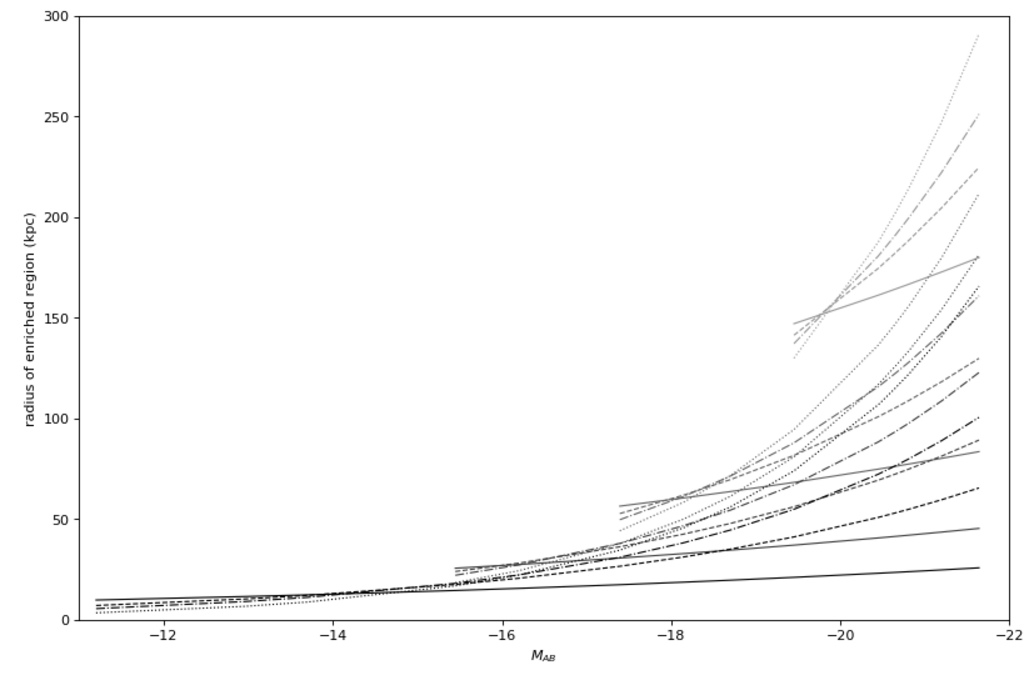
\includegraphics[width=0.85\textwidth]{plots/MgII_few.png}
\caption{Relation between an object's AB magnitude and the expected size of the surrounding \magtwo enriched region. Shades of grey correspond to varying $L_\text{min}/L^*=0.0001,0.001,0.01,0.1$ corresponding to limiting magnitudes of $M_\text{min} = -11.2, -13.7, -16.2, -18.7$, from dark to light. Line shape shows the effect of varying $\beta=0.1,0.23,0.3,0.4$, from continuous to dashed to dotted. Not all lines extend to low luminosities, since those systems are not  enriched if $M_\text{min}$ is high.}
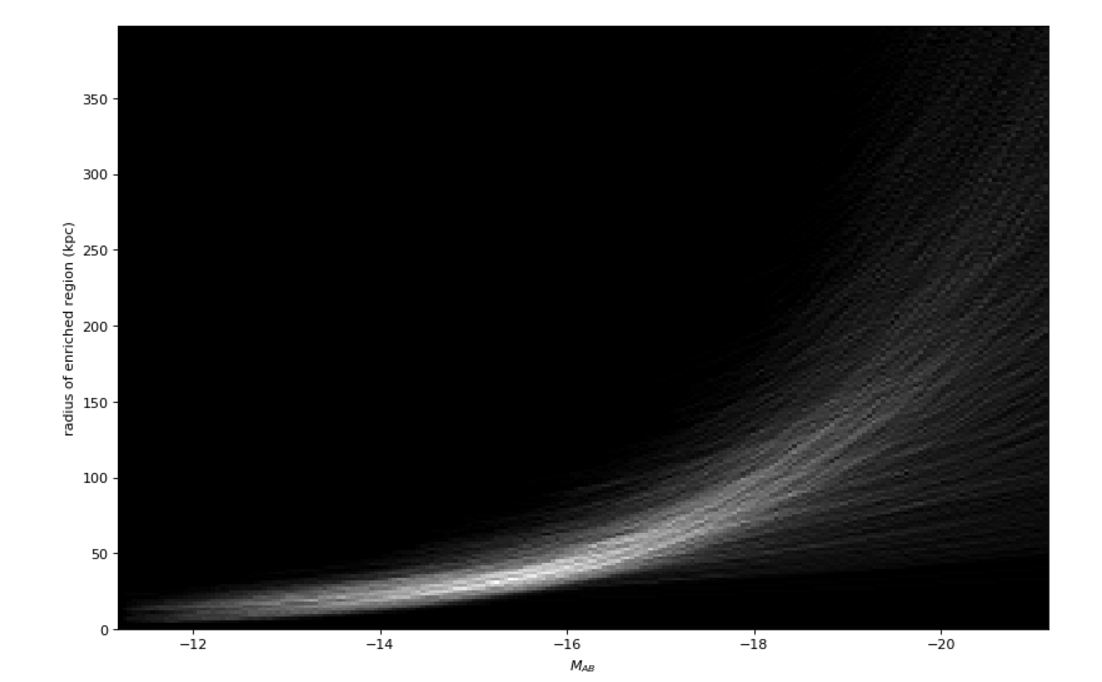
\includegraphics[width=0.9\textwidth]{plots/MgII_range.png}
\caption{Same as Figure 1 for a continuum of models, with all parameters in equation (8) sampled from the allowed ranges given in Tables 1,2 and 3. The regions through which the largest number of models pass are shown in lighter gray, but depend strongly on the choice of prior used for sampling $L_\text{min}$ (and to a lesser extend $\Phi^*$). This figure showcases the full range of models which are compatible with observational constraints, as opposed to establishing which are more likely. However, some models can be excluded based on negative detections of galaxy-absorber pairs towards quasars as discussed in the text.}
\end{figure*}



\subsection{$R(L)$}

The relation $R(L) = R^* (L/L^*)^\beta$ only depends on two parameters $L_{min}$ and $\beta$, with $R^*$ being obtainable from measured quantities using Equation (7). Figure 1 illustrates the effect of varying $L_{min}$ and $\beta$ while keeping all measured parameters fixed at their respective means, while Figure 2 shows the full range of all permitted models in varying parameters within their observational errors. 

This enables us to put constraints on the maximal extent of \magtwo enriched regions as a function of galaxy luminosity. For instance, the enriched regions around galaxies with $M_{AB} = -13$ cannot be larger 25 cMpc in any permissible model. Brighter galaxies with $M_{AB} \sim -18$ similarly cannot possess \magtwo regions larger than 200 cMpc, corresponding to 5.2'' at $z=5$. Indeed, enriched regions above these sizes would lead to higher $dN/dX$ measurements towards high-redshift quasars, or would require fewer galaxies than predicted from measurements of the luminosity function $\Phi(L)$, or extremely low metal enrichment efficiencies ($f<0.5$). The discovery of even a single such instance would put considerable strain on current models, and might require invoking extreme scatter among objects.

Models with large values of $L_\text{min}$, in which only the brightest galaxies produce enriched regions, might already be ruled out by the lack of confirmed galaxy-absorber pairs in observations of fields around quasars. Such models, shown in light gray in Figure 1, predict the galaxies corresponding to line-of-sight absorbers should be both bright and have large radii, and should therefore be readily visible in the surrounding fields. For instance, in models with $M_\text{min} = -18.7$, enriched regions always possess radii $R>140$ cMpc corresponding to 3.6'' on the sky. Assuming random alignment, the probability of confusion of such a galaxy with the central quasar in an instrument such as MUSE is roughly $\lesssim2\%$. A handful of non-detections therefore suffice to confidently constrain $M_\text{min} > -19$.

%Finally, and in my opinion the most useful aspect of this, is the bottom line of $R(L)$. The relation $R=R^* (L/L^*)^\beta$ actually only depends on two parameters: $L_{min}$ and $\beta$, with $R^*$ being obtainable by using our measurements of $dN/dX$. This results in Figure 4, a good summary of all the constraints currently available at $z=5$ with no priors. The figure really shows how good the constraints already are on the sizes of enriched haloes around faint objects: even 1 detection of a halo larger than these limits would raise very serious problems. It also presents an honest perspective on how uncertain the predictions are for the brightest objects. This figure will be extremely useful to observers looking for associated metal absorbers at high redshift.


\subsection{$R_\text{min}$}





%\section{Constraints on parameters}

%We would hope to achieve a posterior like Figure 1 where the shaded area is the 'allowed region' of parameter space based on uncertainties in $\beta, dN/dX$, and the luminosity function.

%\begin{figure}
%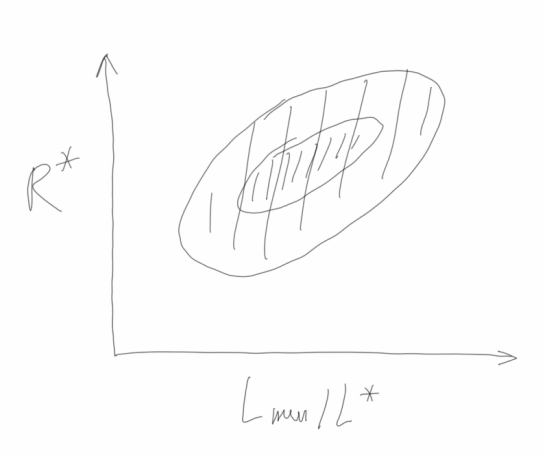
\includegraphics[width=\columnwidth]{plots/sketch.png}
%\caption{What we would like to get}
%\end{figure}


%which means that for each value of $L_{min}$, it is always possible to find a value of $\beta$ which reproduces the observations. Doing things this way, we can input the measurements of dN/dX (with uncertainties) and deduce $R^*$ as a function of $\beta$ and $L_{min}$. The results at $z=5$ are shown in Fig 2.

%\begin{figure}
%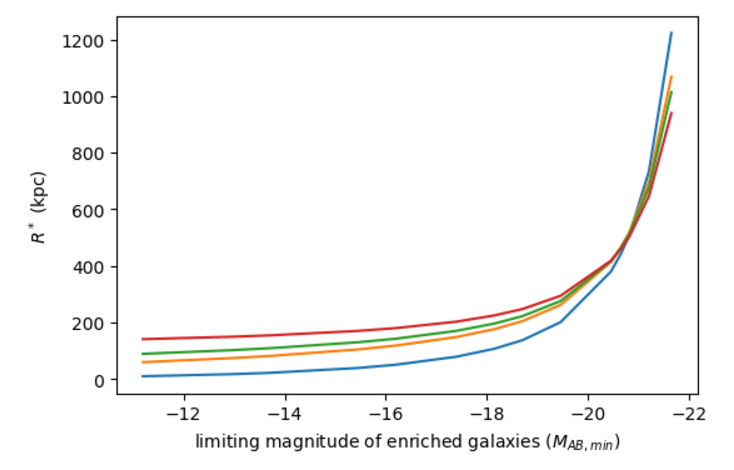
\includegraphics[width=\columnwidth]{plots/degen1.png}
%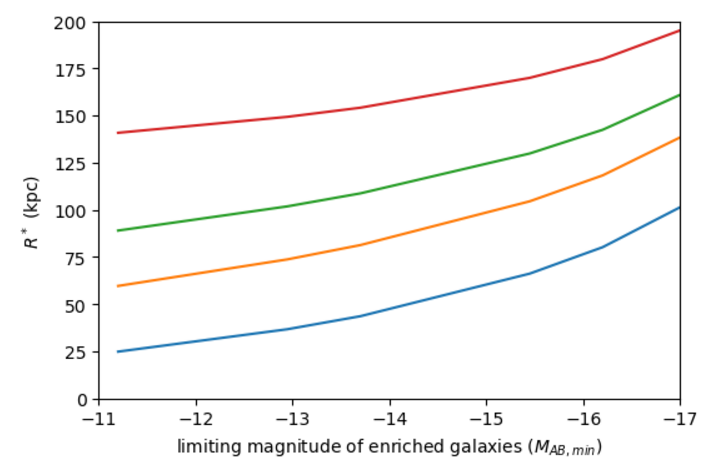
\includegraphics[width=\columnwidth]{plots/degen2.png}
%\caption{What the `posterior' actually looks like: colors blue to red show $\beta=0.1, 0.23, 0.3, 0.4$. Bottom is a zoom on the top panel.}
%\end{figure}

%\newpage

%The problem is that the relation $R = R^* (L/L^*)^\beta$ is extremely uncertain at high redshift. There are no obvious priors as to what this should be, although some scalings of $R^*$ with $(1+z)^3$ have been suggested which we can look into (but this only holds at very low redshift according to the existing litt.). Therefore, a ML analysis would just recover any priors we choose to input into the calculation and isn't particularly justified or necessary.

%There are still a wide range of physical conclusions to be drawn without priors. For instance, the size of the \textit{smallest enriched regions}, $R_{min} = R^* (L_{min}/L^*)^\beta$, is (surprisingly) stable to varying $\beta$ as shown in Fig 3. This is a useful plot for theorists who run simulations: given a choice of halo mass enrichment threshold, it tells the sizes which the simulations should resolve.

\begin{figure}
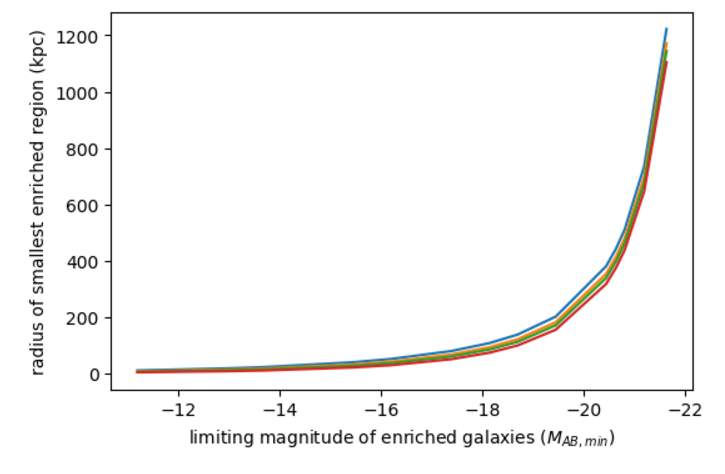
\includegraphics[width=\columnwidth]{plots/smallest1.png}
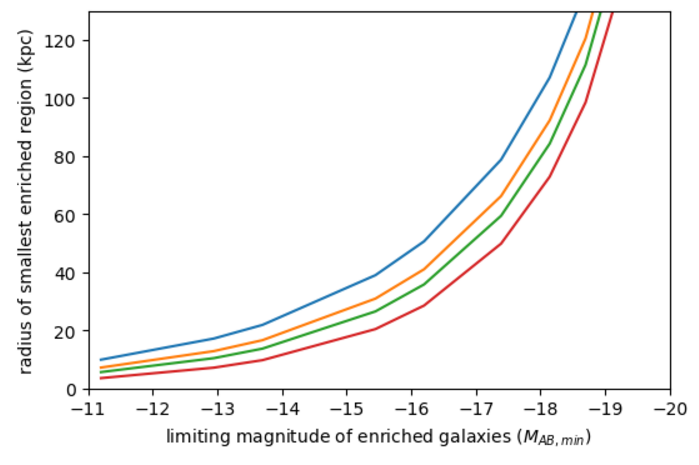
\includegraphics[width=\columnwidth]{plots/smallest2.png}
\caption{Sizes of the smallest enriched haloes: colors blue to red show $\beta=0.1, 0.23, 0.3, 0.4$. Bottom is a zoom on the top panel.}
\end{figure}

%\newpage




%\newpage

%\section{TODO}
%\begin{enumerate}
%\item Do other redshift ranges
%\end{enumerate}

\section{Conclusions}

\bibliographystyle{apj} \bibliography{bibliography}


\end{document}

